\documentclass{beamer}

\usetheme{Madrid} % Other popular themes: default, Madrid, Boadilla, AnnArbor, CambridgeUS
\usecolortheme{default}
\usefonttheme{default}

% Hide navigation symbols
\setbeamertemplate{navigation symbols}{}
\setbeamertemplate{caption}[numbered]

% Title page details: 
\title[Modeling 2D Marshak Waves]{Modeling 2D Marshak Waves}
\subtitle{Optional Subtitle}
\author[Yuval Kochavi]{Yuval Kochavi}
\institute[HUJI]{The Hebrew University of Jerusalem}
\date{June 17, 2026}
% \logo{\includegraphics[height=1cm]{logo-image.png}} % Optional logo

\begin{document}

% Title slide
\begin{frame}
    \titlepage
\end{frame}

% Outline slide
\begin{frame}{Outline}
    \tableofcontents
\end{frame}

% --- Section 1 ---
\section{Describing the Physical system}

\begin{frame}{Photon Transport and Energy Exchange}
    Photon transport (Boltzmann equation):
    \begin{multline}
        \frac{1}{c} \frac{\partial I}{\partial t} + \hat{\Omega} \cdot \nabla I + (\sigma_a(T_m) + \sigma_s(T_m))I = \sigma_a(T_m)B(T_m) \\
        + \frac{\sigma_s(T_m)}{4\pi} \int_{4\pi} I \, d\hat{\Omega} + S(\hat{\Omega}, \vec{r}, t)
    \end{multline}
    
    \vspace{0.5cm}
    Energy exchange between radiation and matter:
    \begin{equation}
        \frac{C_v(T_m)}{c} \frac{\partial T_m}{\partial t} = \sigma_a(T_m) \left( \frac{1}{c} \int_{4\pi} I \, d\hat{\Omega} - aT_m^4 \right)
    \end{equation}
\end{frame}

\begin{frame}{Gray Coupled Equations and LTE}
    We get the "gray" coupled equations:
    \begin{align*}
        \frac{\partial E}{\partial t} - \nabla \cdot \left(\frac{c}{3\sigma} \nabla E\right) &= c\sigma(U - E), \quad \quad U = \mathrm{a} T_m^4, \quad E = \mathrm{a} T_R^4 \\
        \frac{\partial e}{\partial t} &= c\sigma(E - U), \quad \quad e = f T_m^\beta \rho^{-\mu}
    \end{align*}

    Finally, assuming complete thermodynamic equilibrium (CTE) between the radiation field and the material ($T_R = T_m$):
    \begin{equation}
        \frac{\partial T^4}{\partial t} + f \rho^{-\mu}\frac{\partial T^{\beta}}{\partial t} = \nabla \cdot \left(\frac{c}{3\sigma} \nabla (aT^4)\right)
    \end{equation}
    Assuming $\rho f T^\beta \rho^{-\mu} \gg aT^4$ (True until around 3keV):
    \begin{align*}
        f \rho^{-\mu}\frac{\partial T^{\beta}}{\partial t} = \nabla \cdot \left(\frac{c}{3\sigma} \nabla (aT^4)\right)
    \end{align*}
\end{frame}

\begin{frame}{Motivation}
    \begin{figure}
        \centering
        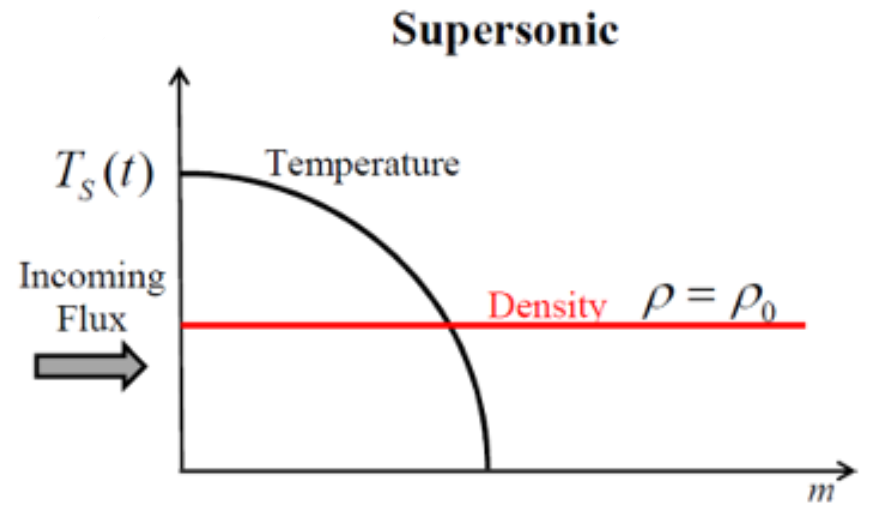
\includegraphics[width=0.45\textwidth]{figures_intreduction/supersonic.png}
    \end{figure}
    
    \vspace{0.2cm}
    \begin{itemize}
        \item Given the material properties equations:
        \begin{equation*}
            e = fT^\beta \rho^{-\mu}, \qquad \frac{1}{\kappa} = gT^\alpha \rho^{-\lambda}
        \end{equation*}
        \item The diffusion coefficient $D$ is not linear.
        \item Because of this, the entire system becomes highly non-linear and hard to solve analytically.
        \item \textbf{Our Motivation:} To build a robust model and fundamentally understand the dynamics of this system.
    \end{itemize}
\end{frame}

% --- Section 2 ---
\section{Marshak Waves Experiments}

\begin{frame}{Marshak Waves Experiments}
    Using a Hohlraum as an x-ray generator, a supersonic heatwave propagates in the low-density foam.
    
    \vspace{0.5cm}
    \begin{columns}
        \begin{column}{0.5\textwidth}
            \centering
            % \includegraphics[width=\textwidth]{figures/laser_pulse_graph.png}
            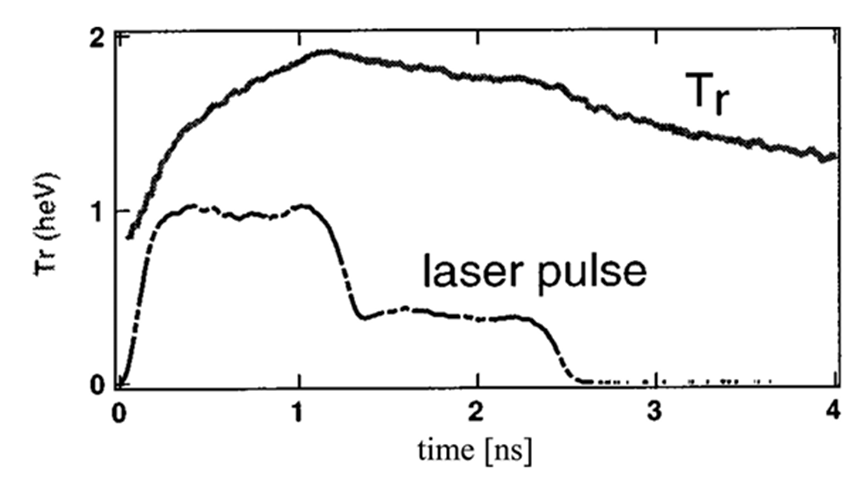
\includegraphics[width=\textwidth]{figures_intreduction/T_drive.png} % Placeholder
        \end{column}
        \begin{column}{0.5\textwidth}
            \centering
            % \includegraphics[width=\textwidth]{figures/hohlraum_diagram.png}
            
\includegraphics[width=\textwidth]{figures_intreduction/setup.png} % Placeholder
        \end{column}
    \end{columns}
\end{frame}

\begin{frame}{Marshak Waves Experiments}
    \begin{columns}
        \begin{column}{0.4\textwidth}
            \centering
            % \includegraphics[width=0.65\textwidth]{figures/radiograph.png} \\
            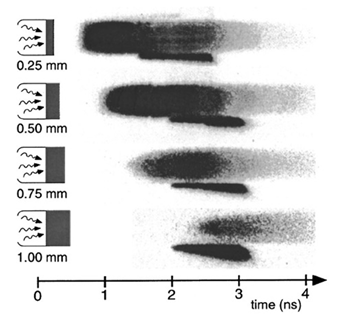
\includegraphics[width=0.72\textwidth]{figures_intreduction/method1.png} \\ % Placeholder
            \vspace{0.1cm}
            % \includegraphics[width=0.65\textwidth]{figures/time_series.png} \\
            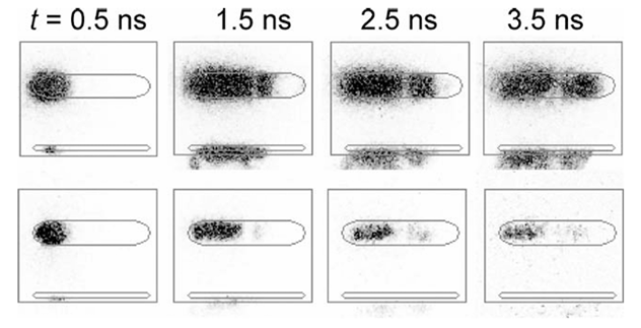
\includegraphics[width=0.72\textwidth]{figures_intreduction/method2.png} \\ % Placeholder
            \vspace{0.1cm}
            % \includegraphics[width=0.65\textwidth]{figures/foam_tube.png}
            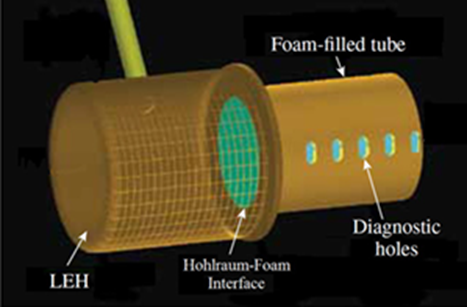
\includegraphics[width=0.72\textwidth]{figures_intreduction/method3.png}    % Placeholder
        \end{column}
        
        \begin{column}{0.1\textwidth}
            \centering
            \Huge $\Rightarrow$ \\
            \vspace{1.5cm}
            \Huge $\Rightarrow$
        \end{column}
        
        \begin{column}{0.5\textwidth}
            \centering
            % \includegraphics[width=0.8\textwidth]{figures/ta2o5_top_graph.png} \\
            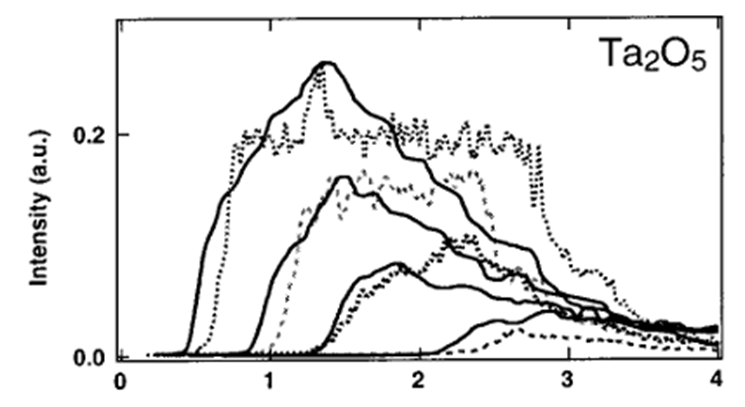
\includegraphics[width=0.9\textwidth]{figures_intreduction/flux.png} \\ % Placeholder
            \vspace{0.2cm}
            % \includegraphics[width=0.8\textwidth]{figures/ta2o5_bottom_graph.png}
            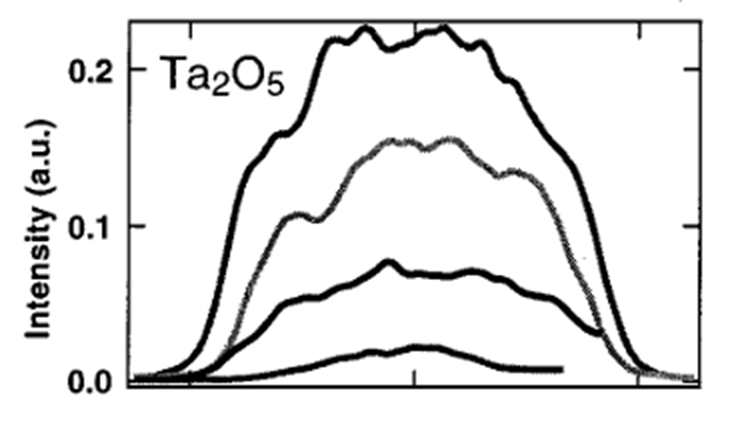
\includegraphics[width=0.9\textwidth]{figures_intreduction/flux_curvature.png}
        \end{column}
    \end{columns}
\end{frame}

\begin{frame}{Experiments tested}
    \begin{table}
        \centering
        \renewcommand{\arraystretch}{1.2}
        \begin{tabular}{llcc}
            \hline \hline
             & & density & temperature \\
            The experiment & foam type & (mg/cc) & (eV) \\
            \hline
            Massen \textit{et al.} & $\mathrm{C}_{11}\mathrm{H}_{16}\mathrm{Pb}_{0.3852}$ & 80 & 100--150 \\
            Back \textit{et al.} & $\mathrm{SiO}_2$, $\mathrm{Ta}_2\mathrm{O}_5$ & 10--50 & 85--190 \\
            Xu \textit{et al.} & \begin{tabular}{@{}l@{}}$\mathrm{C}_6\mathrm{H}_{12}$, \\ $\mathrm{C}_6\mathrm{H}_{12}\mathrm{Cu}_{0.394}$\end{tabular} & 50 & 160 \\
            Ji-Yan \textit{et al.} & $\mathrm{C}_8\mathrm{H}_8$ & 160 & 175 \\
            Rosen and Keiter \textit{et al.} & \begin{tabular}{@{}l@{}}$\mathrm{C}_{15}\mathrm{H}_{20}\mathrm{O}_6$, \\ $\mathrm{C}_{15}\mathrm{H}_{20}\mathrm{O}_6\mathrm{Au}_{0.172}$\end{tabular} & 45--70 & 200--210 \\
            Moore \textit{et al.} & $\mathrm{SiO}_2$, $\mathrm{C}_8\mathrm{H}_7\mathrm{Cl}$ & 90--120 & 310 \\
            Courtois \textit{et al.} & $\mathrm{SiO}_2$ & 19 -- 29 & 170 \\
            \hline \hline
        \end{tabular}
    \end{table}
\end{frame}

% --- Section 3 ---
\section{1.5D model}

\begin{frame}
    \vfill
    \begin{center}
        \Huge \textbf{1.5D model}
    \end{center}
    \vfill
\end{frame}

\begin{frame}{HR Model - Governing Equations}
    The "Black" diffusion equation (neglecting radiation energy density $\frac{\partial E}{\partial t} \to 0$):
    \begin{equation*}
        \underbrace{\frac{\partial E}{\partial t}}_{\to 0} + \frac{\partial e}{\partial t} = \frac{\partial}{\partial x} \left( \frac{c}{ 3 \rho \kappa} \frac{\partial (aT^4)}{\partial x} \right)
    \end{equation*}

    With specific energy and opacity models:
    \begin{equation*}
        e = fT^\beta \rho^{-\mu}, \qquad \frac{1}{\kappa} = gT^\alpha \rho^{-\lambda}
    \end{equation*}
    where $f, \mu, g, \lambda, \alpha, \beta$ are material-dependent parameters. 
    
    HR solved the diffusion equation using perturbation theory and found some interesting results. 
\end{frame}

\begin{frame}{HR Model - Heat Front Solution}
    The heat front position $x_F(t)$ is given by:
    \begin{equation*}
        \boldsymbol{x_F^2(t) = \frac{2 + \varepsilon}{1 - \varepsilon} C H^{-\varepsilon}(t) \int_0^t H(t') \, dt'}
    \end{equation*}
    
    where:
    \begin{equation*}
        C = \frac{16g\sigma_{SB}}{3f(4+\alpha)} \rho^{2-\mu-\lambda}; \quad \varepsilon = \frac{\beta}{4+\alpha}
    \end{equation*}
    \begin{equation*}
        H(t) = T_s^{4+\alpha}(t)
    \end{equation*}
    where $T_s$ is the surface temperature at $x=0$.

\end{frame}

\begin{frame}{HR 1D Model Limitations}
    HR misses the real experimental results of Back et al. by a factor of 2!
    
    \vspace{0.2cm}
    \begin{figure}
        \centering
        
\includegraphics[width=0.7\textwidth]{figures_1.5model/HR.png}
    \end{figure}
\end{frame}

\subsection{1D effects}
\begin{frame}
    \vfill
    \begin{center}
        \Huge \textbf{1.5D model}

        \vspace{0.5cm}
        \Large \textbf{1D effects}
    \end{center}
    \vfill
\end{frame}

\begin{frame}{Marshak Boundary Condition: $T_D \neq T_s$}
    \begin{itemize}
        \item Assuming $T_s = T_D$ overestimates the wave speed.
        \item Instead, energy conservation at the boundary requires:
        \begin{equation*}
            \sigma_{SB} T_D^4(t) = \sigma_{SB} T_s^4(t) + \frac{F(0,t)}{2}
        \end{equation*}
        where $F(0,t)$ is the net flux entering the foam. 
    \end{itemize}
\end{frame}

\begin{frame}{Marshak Boundary Condition: $T_D \neq T_s$}
    Applying the Marshak boundary condition slows the propagation front significantly:
    
    \vspace{0.2cm}
    \begin{figure}
        \centering
        
\includegraphics[width=0.7\textwidth]{figures_1.5model/marshak.png}
    \end{figure}
\end{frame}

\subsection{2D effects}
\begin{frame}
    \vfill
    \begin{center}
        \Huge \textbf{1.5D model}

        \vspace{0.5cm}
        \Large \textbf{2D effects}
    \end{center}
    \vfill
\end{frame}

\begin{frame}{Energy Wall Loss}
    \begin{itemize}
        \item Energy is lost from the foam into the tube walls.
        \item Can be modeled for different wall materials: \textbf{Gold}, \textbf{Copper}, \textbf{Beryllium}, and \textbf{Vacuum} .
        \item For \textbf{Gold}:
        \begin{equation*}
            E_{\mathrm{gold}}(t) = 0.59\, T_s^{3.35}\, [t - t_0(x)]^{0.59} \quad [\mathrm{hJ/mm^2}]
        \end{equation*}
        where $t_0(x)$ is the front arrival time at position $x$.
    \end{itemize}
\end{frame}

\begin{frame}{Energy Wall Loss}
    Including wall loss reduces the front velocity:
    
    \vspace{0.2cm}
    \begin{figure}
        \centering
        
\includegraphics[width=0.7\textwidth]{figures_1.5model/wall_loss.png}
    \end{figure}
\end{frame}

\begin{frame}{Wall Ablation}
    \begin{itemize}
        \item High-Z wall material (e.g. Gold) absorbs energy and ablates inward into the foam.
        \item \textbf{Changing Foam Radius}: The inlet and tube radius shrink, reducing the heat wave cross-section.
        \item \textbf{Changing Foam Density}: The ablated wall material compresses and densifies the adjacent foam.
        \item Both effects must be incorporated to model the dynamic tube geometry.
    \end{itemize}
\end{frame}

\begin{frame}{Wall Ablation}
    Inward wall ablation compressively densifies the foam, which significantly slows down propagation:
    
    \vspace{0.2cm}
    \begin{figure}
        \centering
        
\includegraphics[width=0.7\textwidth]{figures_1.5model/denser_foam.png}
    \end{figure}
\end{frame}

\begin{frame}{Effective Mean Free Path}
    When $\lambda_R \ge 2R$, wall collisions control the transport instead of diffusion.

    Can be modeled as:
    \begin{equation*}
        \frac{1}{\lambda_{\mathrm{eff}}} = \frac{1}{\lambda_R} + \frac{1}{2R}
    \end{equation*}
    where $\lambda_R$ is the Ross Mean Free Path.
    
    \vspace{0.2cm}
    A smoother transition is defined using the generalized power mean:
    \begin{equation*}
        \lambda_{\mathrm{eff}} = \left( (2R)^{-n} + \lambda_{\mathrm{R}}^{-n} \right)^{-1/n}
    \end{equation*}
    where $n$ controls the "tightness" of the transition.
\end{frame}

\begin{frame}{Effective Mean Free Path}
    Including the effective mean free path correction matches the simulation to the experimental data at early times:
    
    \vspace{0.2cm}
    \begin{figure}
        \centering
        
\includegraphics[width=0.7\textwidth]{figures_1.5model/lam_eff.png}
    \end{figure}
\end{frame}

\begin{frame}{Comparison to many experiments}
    \begin{columns}
        \begin{column}{0.48\textwidth}
            \centering
                
\includegraphics[width=0.78\textwidth]{figures_1.5model/C8H7Cl.png}

            {\scriptsize \textit{Moore at el. JQSRT, (2015)}}
        \end{column}
        \begin{column}{0.48\textwidth}
            \centering
                
\includegraphics[width=0.78\textwidth]{figures_1.5model/Ta2O5.png}

            {\scriptsize \textit{Back at el. POP, (2000)}}
        \end{column}
    \end{columns}
    \vspace{0.1cm}
    \begin{columns}
        \begin{column}{0.48\textwidth}
            \centering
                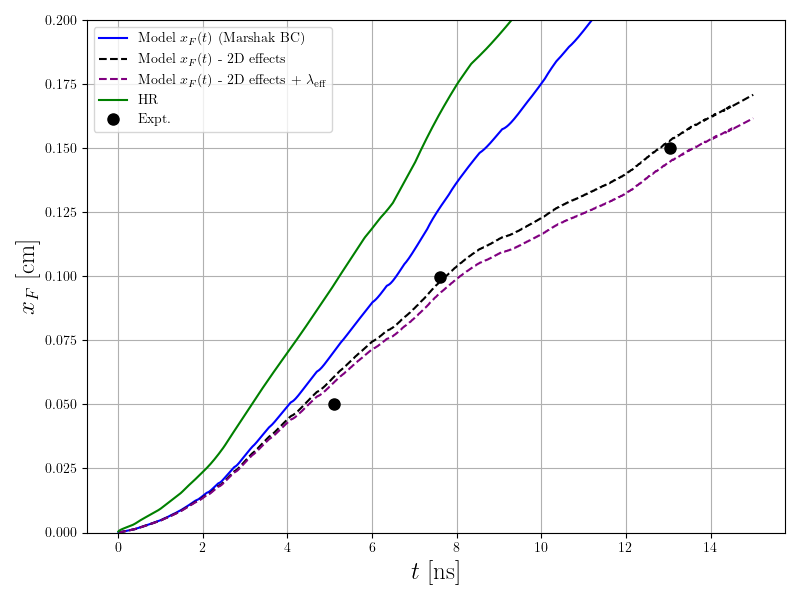
\includegraphics[width=0.78\textwidth]{figures_1.5model/SiO2_low_energy.png}

            {\scriptsize \textit{Back at el. PRL, (2000)}}
        \end{column}
        \begin{column}{0.48\textwidth}
            \centering
                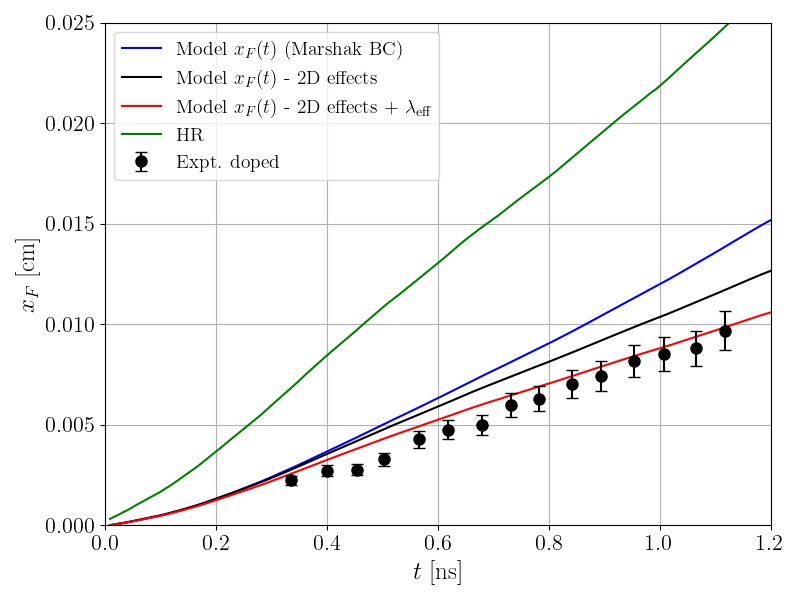
\includegraphics[width=0.78\textwidth]{figures_1.5model/Ji-Yan.png}

            {\scriptsize \textit{Ji-Yan at el. CPB, (2010)}}
        \end{column}
    \end{columns}
\end{frame}

\section{Full 2D model}
\subsection{Modeling the front curvature}
\begin{frame}
    \vfill
    \begin{center}
        \Huge \textbf{Full 2D model}

        \vspace{0.5cm}
        \large \textbf{Modeling the front curvature}
    \end{center}
    \vfill
\end{frame}

\begin{frame}{Understanding the front curvature}
    Hurricane \& Hammer (2006) solved the laplace equation (assumed constant opacity and neglected $e$):
    \begin{equation*}
        \underbrace{\frac{\partial e}{\partial t}}_{\to 0} = \frac{4}{3} \nabla \cdot \left( \frac{1}{ \rho \kappa} \nabla (T^4) \right)
    \end{equation*}
    and got the 2D front in Cartesian coordinates (where $\varepsilon = \frac{3}{4}\rho\kappa L (1-a)$):
    \begin{equation*}
        x_F(y,t) = \frac{L}{\varepsilon} \cosh^{-1}\left(1 + \frac{D\varepsilon t}{L^2}\right) \cos\left(\frac{\sqrt{\varepsilon}}{L}y\right) + \text{HOT}
    \end{equation*}

    \begin{figure}
        \centering
        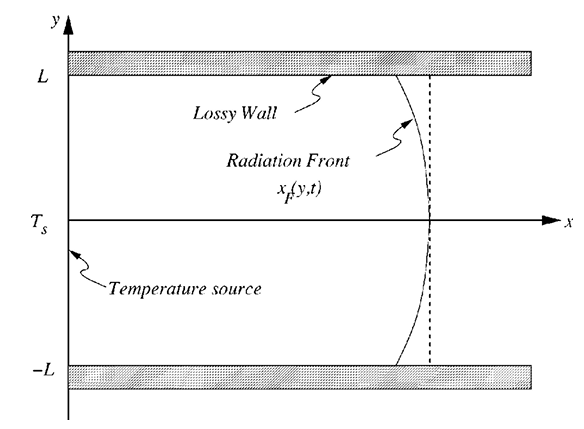
\includegraphics[height=0.4\textheight]{figures_intreduction/hurricane.png}
    \end{figure}
\end{frame}

\begin{frame}{Cylinder Coordinates}
    \begin{columns}
        \begin{column}{0.58\textwidth}
            The model was re-developed in cylindrical coordinates (French group) to match cylindrical geometries:
            \begin{equation*}
                x_F(r,t) = \frac{1}{\kappa_0} \cosh^{-1}\left(1 + \frac{D\kappa_0^2 t}{2}\right) J_0(\kappa_0 r) + \text{HOT}
            \end{equation*}
            
            \textbf{Planar $\longleftrightarrow$ Cylindrical Analogy}: $\cos(k y) \longleftrightarrow J_0(\kappa r)$
            \vspace{0.1cm}
            For small $\varepsilon$:
            \begin{equation*}
                \kappa_0 \approx \frac{\sqrt{2\varepsilon}}{R}, \quad \varepsilon = \frac{3}{4}\rho\kappa R (1-a)
            \end{equation*}
            where $a$ is the wall albedo.
        \end{column}
        \hfill
        \begin{column}{0.4\textwidth}
            \centering
            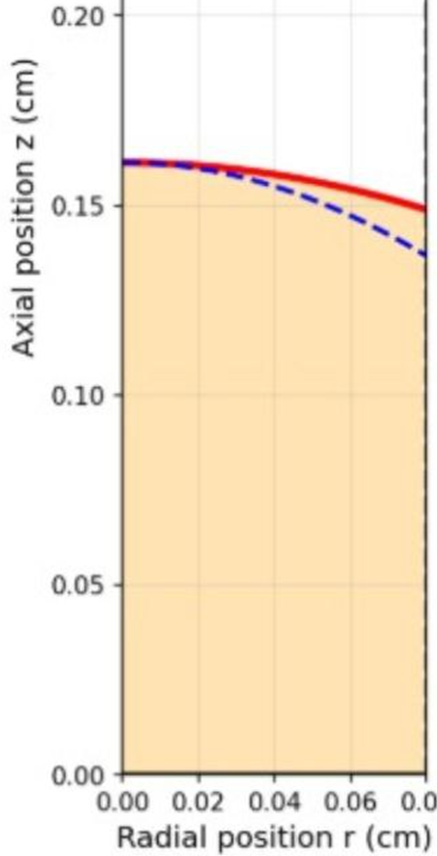
\includegraphics[width=0.7\textwidth]{2D_model/cylinder_vs_cartezian.png}
        \end{column}
    \end{columns}
\end{frame}

\begin{frame}{Applying on our model: Dynamic Albedo}
    \begin{columns}
        \begin{column}{0.55\textwidth}
            Until now, wall albedo was treated as a constant parameter. We update it dynamically in time:
            \begin{equation*}
                \alpha(t) = \frac{F_{\text{out, wall}}}{F_{\text{in,wall}}} = \frac{\sigma_{SB}T_{s,interface}^4 - \frac{dE_{\text{wall}}}{dt}/2}{\sigma_{SB}T_{s,interface}^4+\frac{dE_{\text{wall}}}{dt}/2}
            \end{equation*}
            This provides a much more physical description of the energy reflection.
            
            \vspace{0.2cm}
            where the curvature goes as $J_0\left(\frac{\sqrt{2\varepsilon(t)}}{R}\right)$, and $\varepsilon(t)$ scales with $(1 - \alpha(t))$.
        \end{column}
        \hfill
        \begin{column}{0.42\textwidth}
            \centering
            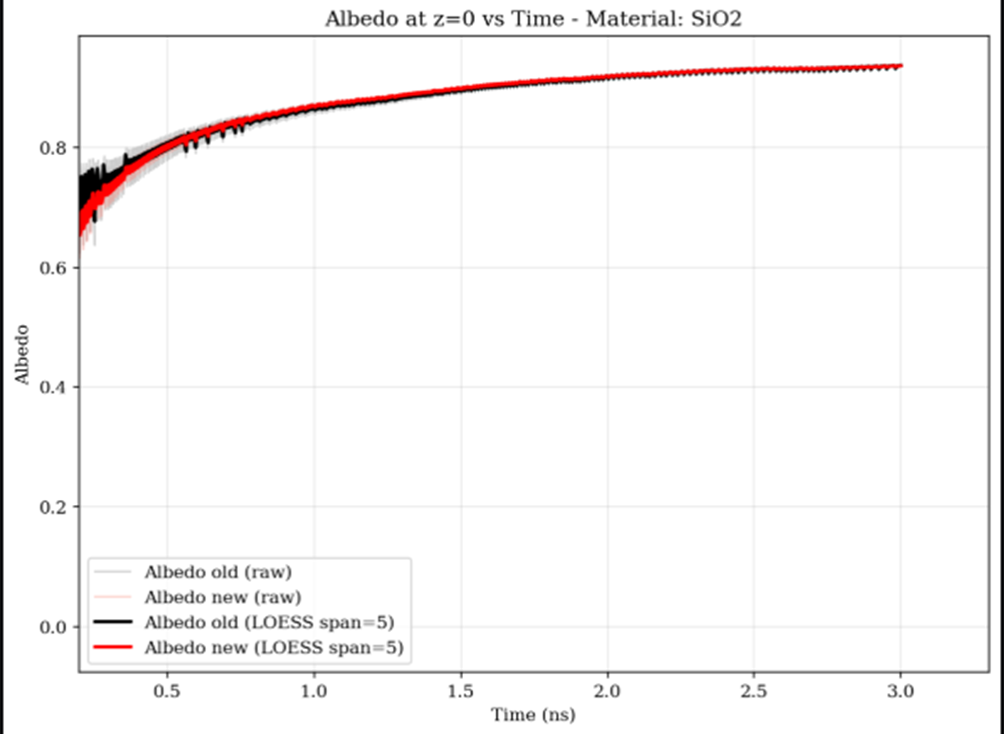
\includegraphics[width=\textwidth]{2D_model/albedo.png}
        \end{column}
    \end{columns}
\end{frame}

\begin{frame}
    \vfill
    \begin{center}
        \Huge \textbf{Problem: the longitudinal front is way off!}
    \end{center}
    \vfill
\end{frame}

\begin{frame}
    \vfill
    \begin{center}
        \Huge \textbf{Luckily, we have a direct longitudinal position:}
        
        \vspace{0.8cm}
        \huge
        \begin{equation*}
            \boldsymbol{x_F(r,t) = x_{\text{1.5D}}(t) \cdot J_0\left(\kappa_0 (t) r\right)}
        \end{equation*}
    \end{center}
    \vfill
\end{frame}


\subsection{Comparing to 2D supersonic diffusion simulation}
\begin{frame}
    \vfill
    \begin{center}
        \Huge \textbf{Full 2D model}

        \vspace{0.5cm}
        \large \textbf{Comparing to 2D supersonic Diffusion Simulation}
    \end{center}
    \vfill
\end{frame}


\begin{frame}{Gold coating - SiO2}
    \begin{figure}
        \centering
            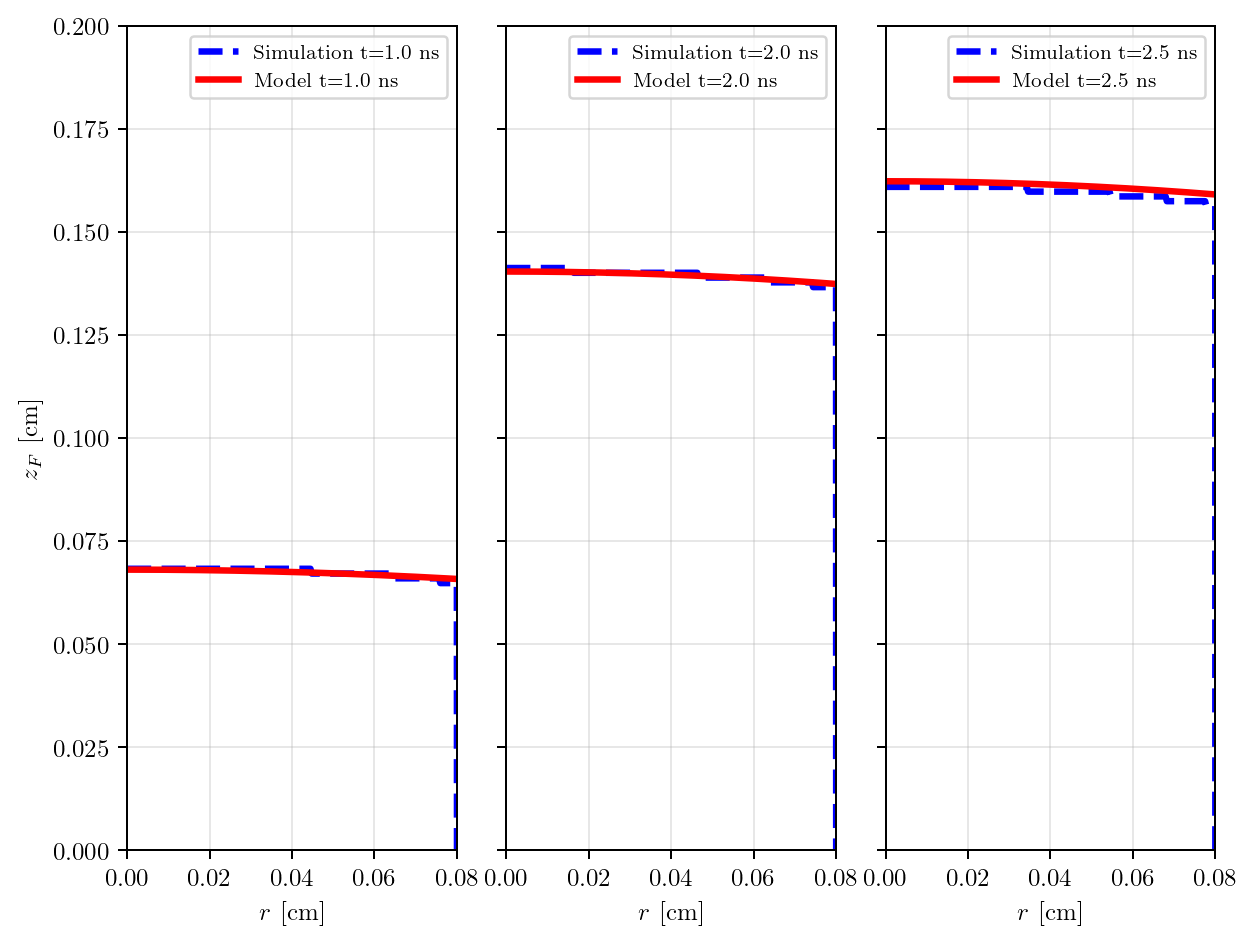
\includegraphics[width=0.8\textwidth]{2D_model/front_surface_gold.png}
    \end{figure}
\end{frame}

\begin{frame}{100 times transparenter Gold coating - SiO2}
    \begin{figure}
        \centering
        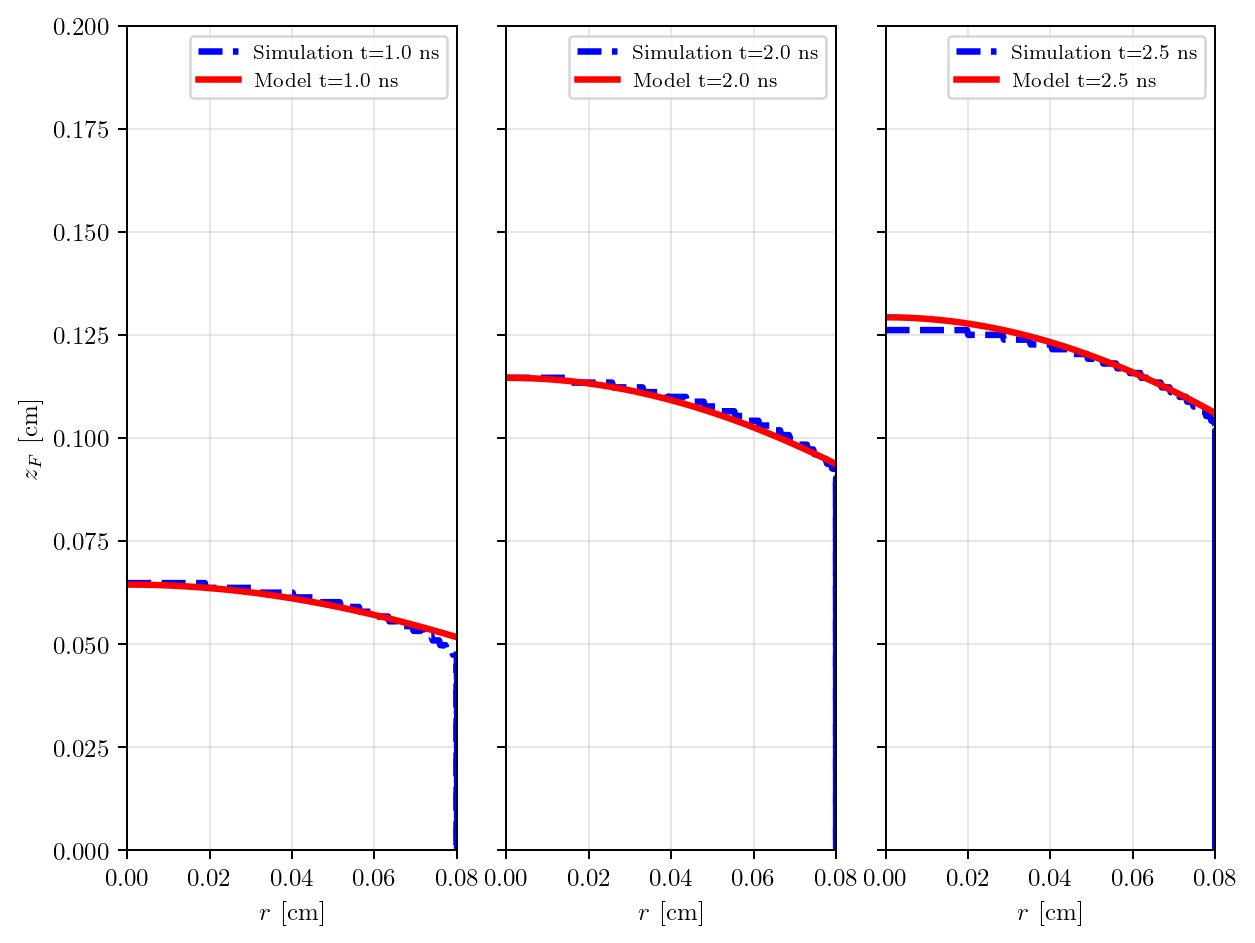
\includegraphics[width=0.8\textwidth]{2D_model/front_surface_gold100.png}
    \end{figure}
\end{frame}

\begin{frame}{Copper - SiO2}
    \begin{figure}
        \centering
        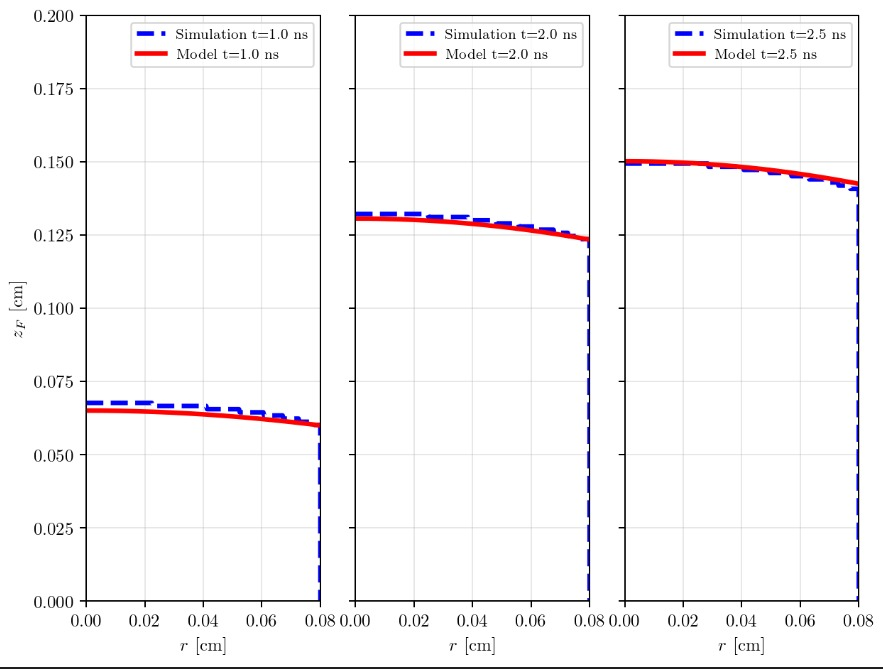
\includegraphics[width=0.8\textwidth]{2D_model/front_surface_copper.png}
    \end{figure}
\end{frame}

\begin{frame}{Be - SiO2}
    \begin{figure}
        \centering
        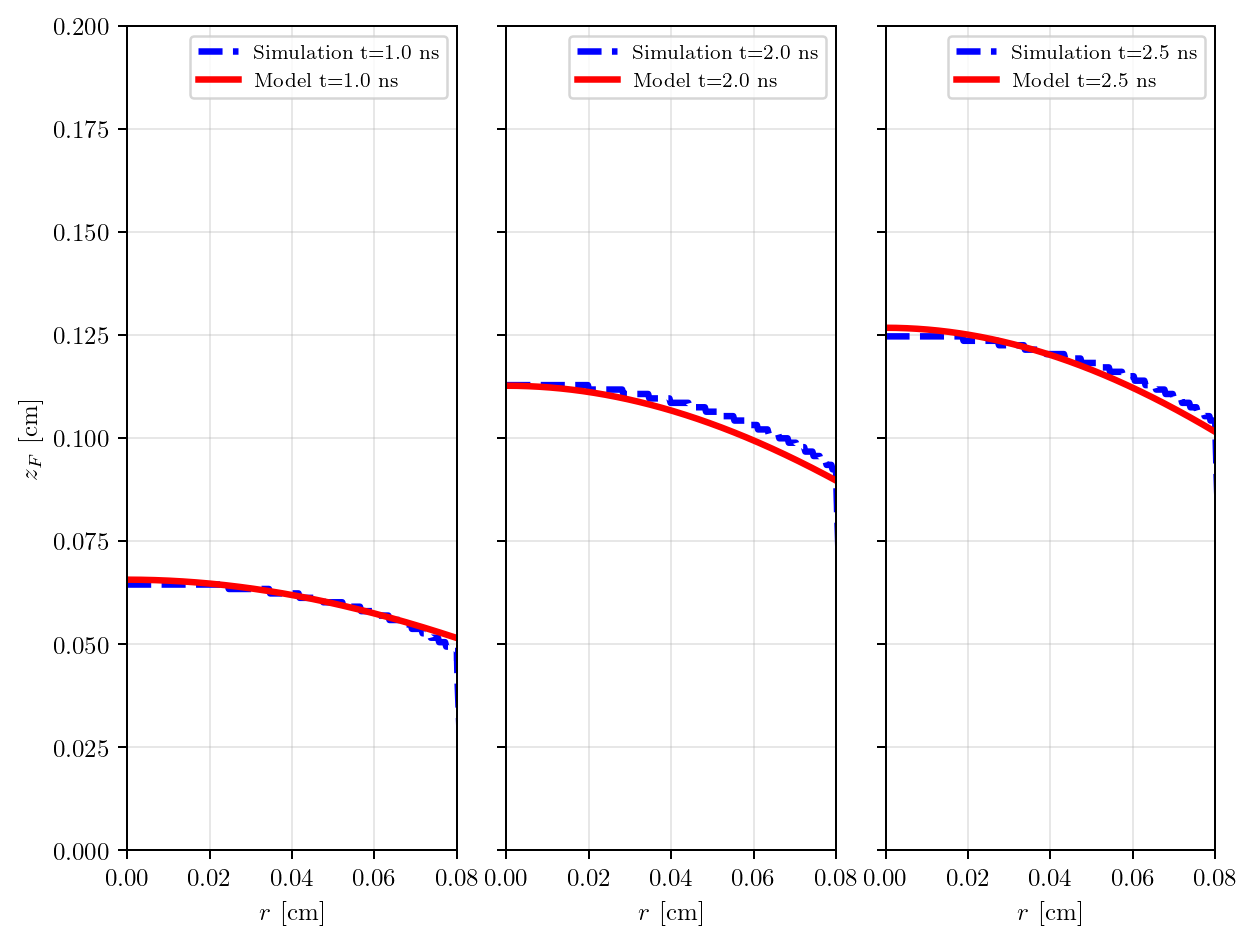
\includegraphics[width=0.8\textwidth]{2D_model/front_surface_be.png}
    \end{figure}
\end{frame}

\begin{frame}{Vacuum - SiO2}
    \begin{figure}
        \centering
        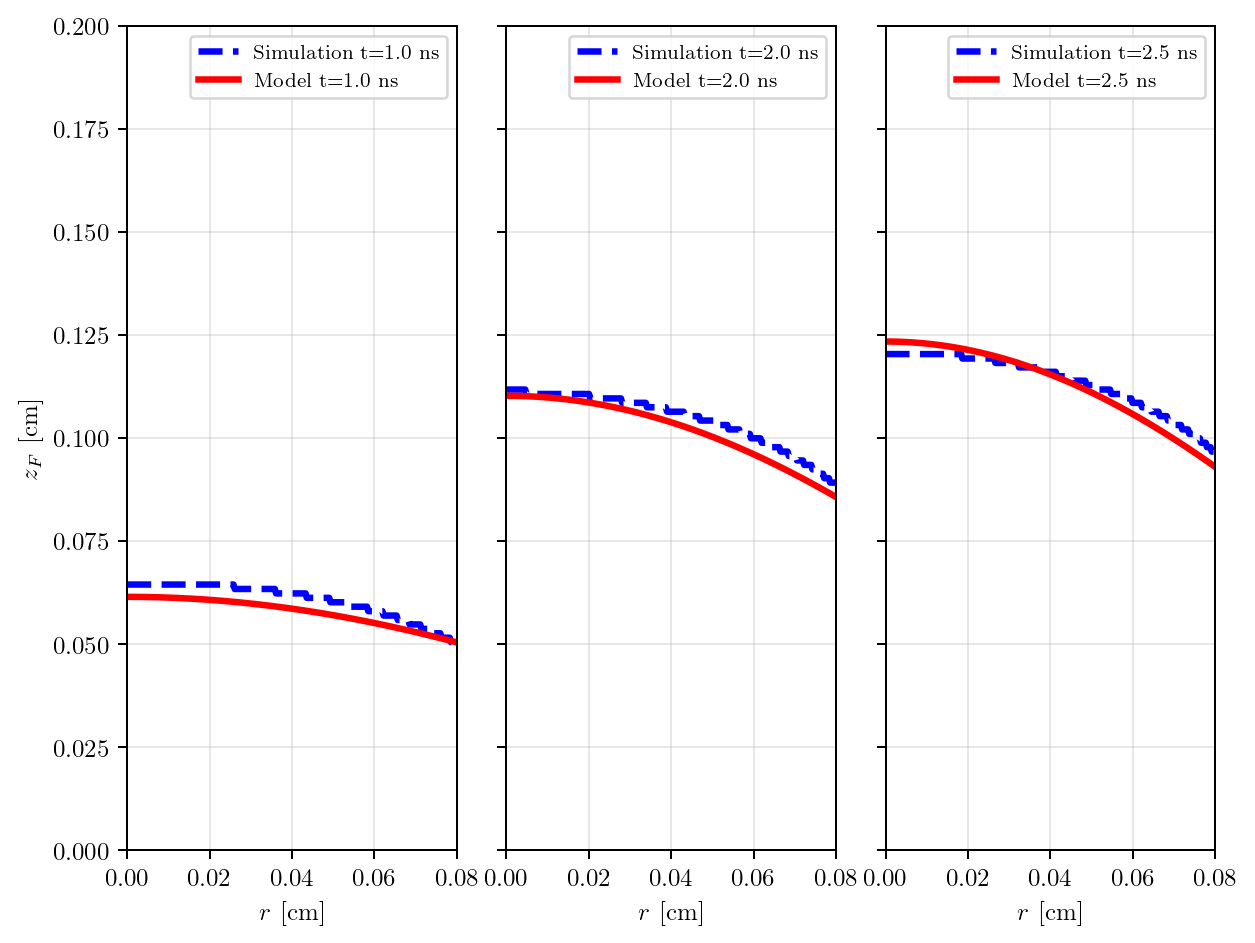
\includegraphics[width=0.8\textwidth]{2D_model/front_surface_vacuum.png}
    \end{figure}
\end{frame}

\subsection{A full 2D Temperature distribution}
\begin{frame}
    \vfill
    \begin{center}
        \Huge \textbf{Full 2D model}

        \vspace{0.5cm}
        \large \textbf{A full 2D Temperature distribution}
    \end{center}
    \vfill
\end{frame}

\begin{frame}{A full 2D Temperature distribution}
    One can use the Heyney profile:
    \begin{equation*}
        T(z,r,t) \approx T_S(t) \left[ 1 - \frac{z}{z_F(r,t)} \right]^{\frac{1}{4+\alpha-\beta}}
    \end{equation*}

    \vspace{0.3cm}
    \begin{columns}
        \begin{column}{0.3\textwidth}
            \centering
            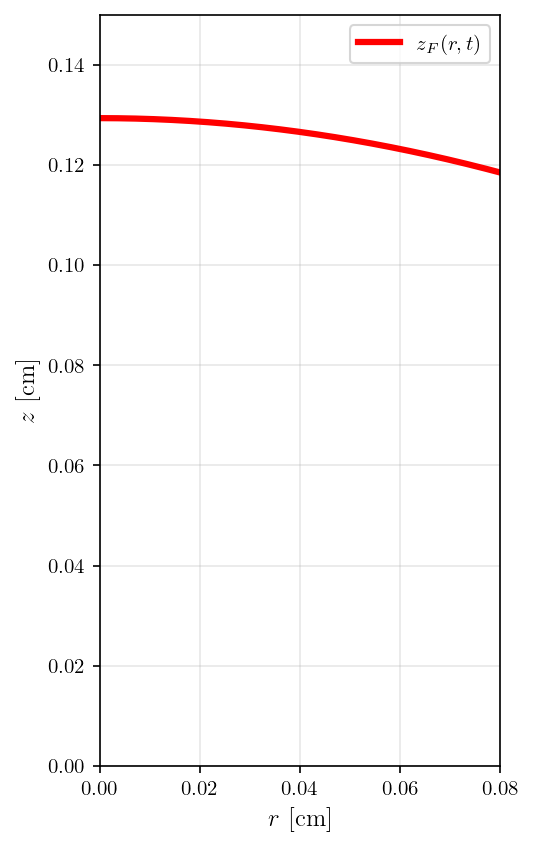
\includegraphics[width=\textwidth]{2D_model/2D_front_spatial.png} \\
            \vspace{0.1cm}
        \end{column}
        \begin{column}{0.12\textwidth}
            \centering
            \Huge $\Rightarrow$
        \end{column}
        \begin{column}{0.35\textwidth}
            \centering
            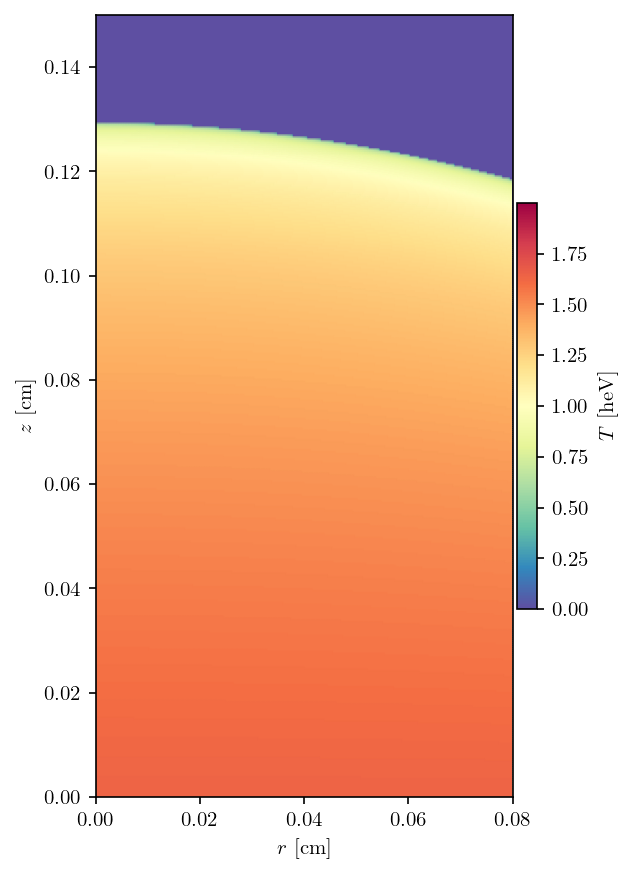
\includegraphics[width=\textwidth]{2D_model/temperature_heatmap_2D(gold wall loss).png} \\
            \vspace{0.1cm}
        \end{column}
    \end{columns}
\end{frame}

\begin{frame}{2D Temperature Distribution — Moore ($\mathrm{C}_8\mathrm{H}_7\mathrm{Cl}$)}
    \begin{columns}
        \begin{column}{0.4\textwidth}
                Side-by-side comparison of the 2D temperature distribution at $t = 3.72$ ns:
                \begin{itemize}
                    \item \textbf{Left}: Diffusion simulation taken from \textit{Moore at el. JQSRT, (2015)}.
                    \item \textbf{Right}: Our full 2D analytical model.
                \end{itemize}
        \end{column}
        \begin{column}{0.6\textwidth}
            \centering
            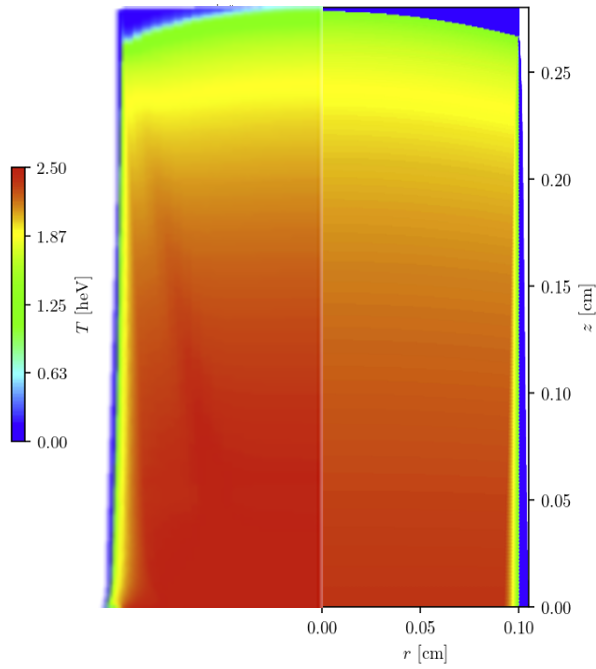
\includegraphics[height=0.9\textheight]{2D_model/moore_simulation.png}
        \end{column}
    \end{columns}
\end{frame}

\begin{frame}{2D Temp. Distribution — Back SiO2 ($1.0$ ns)}
    \begin{columns}
        \begin{column}{0.4\textwidth}
                Side-by-side comparison of the 2D temperature distribution at $t = 1.0$ ns:
                \begin{itemize}
                    \item \textbf{Left}: Implicit Monte Carlo (IMC) simulation of \textit{Back et al. POP, (2000)} experiment.
                    \item \textbf{Right}: Our full 2D analytical model with $\lambda_{\text{eff}} = 1.5$ correction.
                \end{itemize}
        \end{column}
        \begin{column}{0.6\textwidth}
            \centering
            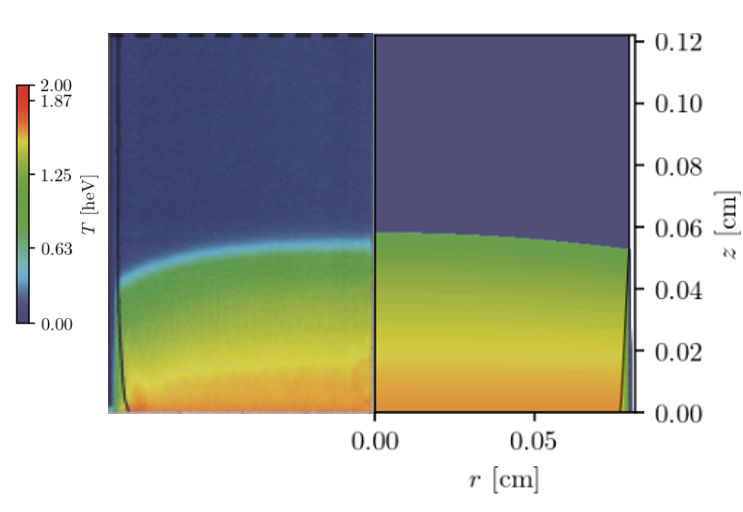
\includegraphics[height=0.55\textheight]{2D_model/back_1ns.png}
        \end{column}
    \end{columns}
\end{frame}

\begin{frame}{2D Temp. Distribution — Back SiO2 ($2.0$ ns)}
    \begin{columns}
        \begin{column}{0.4\textwidth}
                Side-by-side comparison of the 2D temperature distribution at $t = 2.0$ ns:
                \begin{itemize}
                    \item \textbf{Left}: Implicit Monte Carlo (IMC) simulation of \textit{Back et al. POP, (2000)} experiment.
                    \item \textbf{Right}: Our full 2D analytical model with $\lambda_{\text{eff}} = 1.5$ correction.
                \end{itemize}
        \end{column}
        \begin{column}{0.6\textwidth}
            \centering
            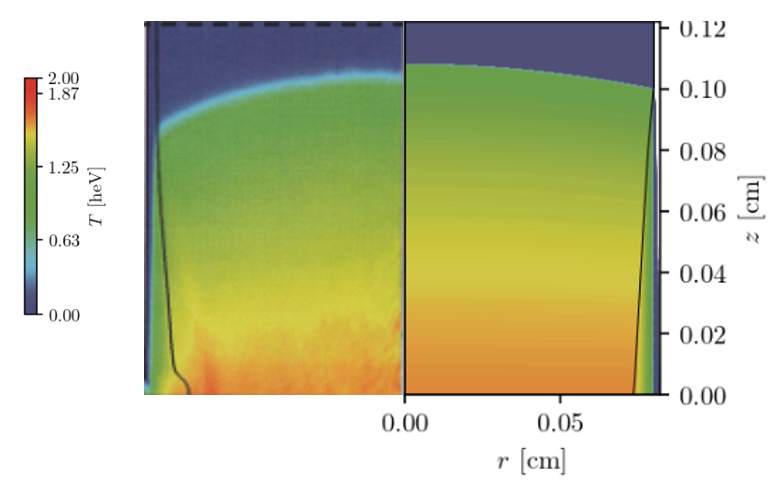
\includegraphics[height=0.5\textheight]{2D_model/back_2ns.png}
        \end{column}
    \end{columns}
\end{frame}

\begin{frame}{2D Temp. Distribution — Back SiO2 ($2.5$ ns)}
    \begin{columns}
        \begin{column}{0.4\textwidth}
                Side-by-side comparison of the 2D temperature distribution at $t = 2.5$ ns:
                \begin{itemize}
                    \item \textbf{Left}: Implicit Monte Carlo (IMC) simulation of \textit{Back et al. POP, (2000)} experiment.
                    \item \textbf{Right}: Our full 2D analytical model with $\lambda_{\text{eff}} = 1.5$ correction.
                \end{itemize}
        \end{column}
        \begin{column}{0.6\textwidth}
            \centering
            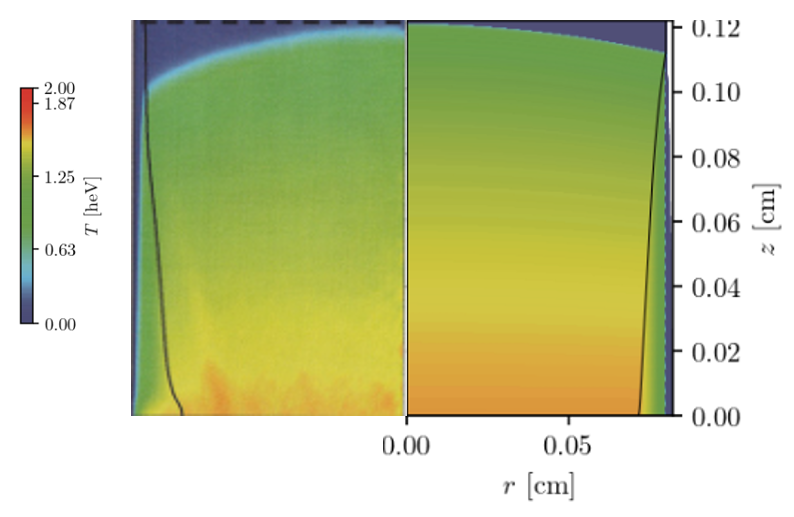
\includegraphics[height=0.53\textheight]{2D_model/back_2.5ns.png}
        \end{column}
    \end{columns}
\end{frame}

\begin{frame}{Flux Curvature Comparison - Back SiO2 PRL}
    \begin{columns}
        \begin{column}{0.37\textwidth}
            \centering
            
\includegraphics[width=\textwidth]{2D_model/prl_T4.png} \\
            \vspace{0.2cm}
            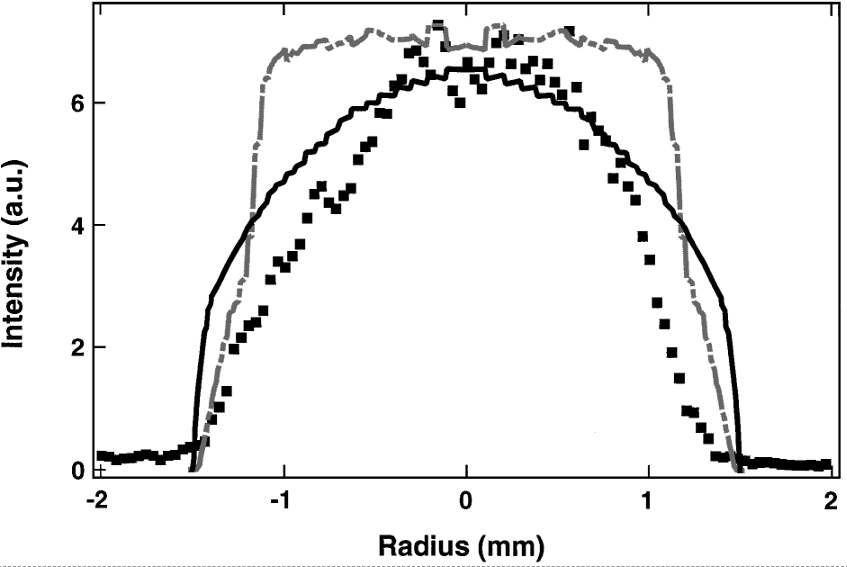
\includegraphics[width=0.9\textwidth]{2D_model/prl.png}
            {\scriptsize \textit{Back at el. POP, (2000)}}
        \end{column}
        \begin{column}{0.1\textwidth}
            \centering
            \Huge $\Rightarrow$
        \end{column}
        \begin{column}{0.6\textwidth}
            \centering
            
\includegraphics[width=\textwidth]{2D_model/back_prl_curve.png}
        \end{column}
    \end{columns}
\end{frame}

\begin{frame}{Flux Curvature Comparison - Back Ta2O5 POP}
    \begin{columns}
        \begin{column}{0.37\textwidth}
            \centering
            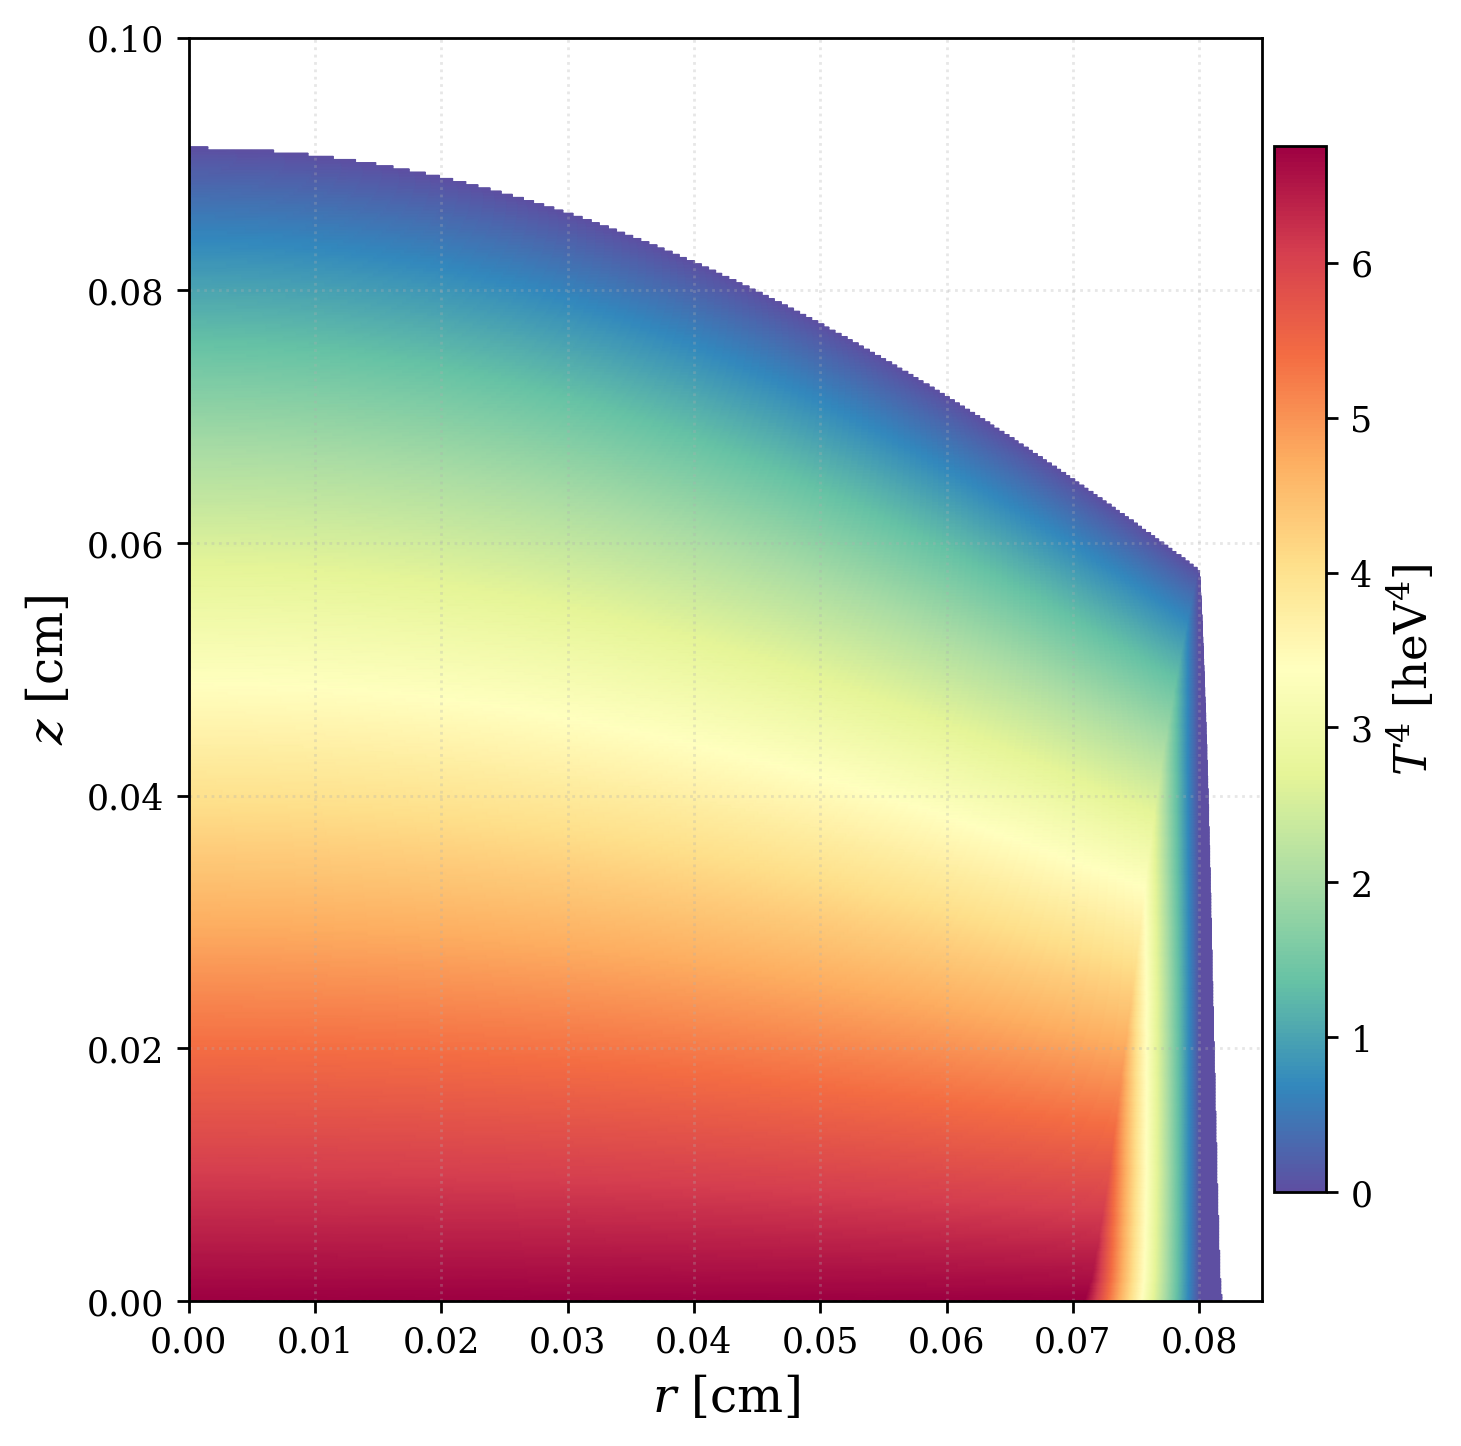
\includegraphics[width=\textwidth]{2D_model/T4_spatial_heatmap_2.0ns.png} \\
            \vspace{0.2cm}
            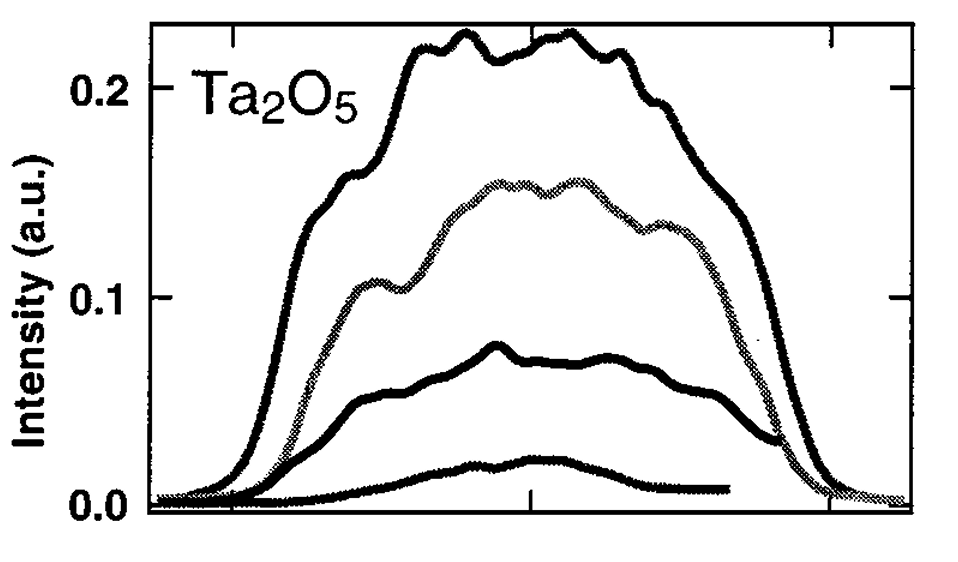
\includegraphics[width=0.9\textwidth]{2D_model/Ta2O5_intensity.png}
            {\scriptsize \textit{Back at el. POP, (2000)}}
        \end{column}
        \begin{column}{0.1\textwidth}
            \centering
            \Huge $\Rightarrow$
        \end{column}
        \begin{column}{0.6\textwidth}
            \centering
            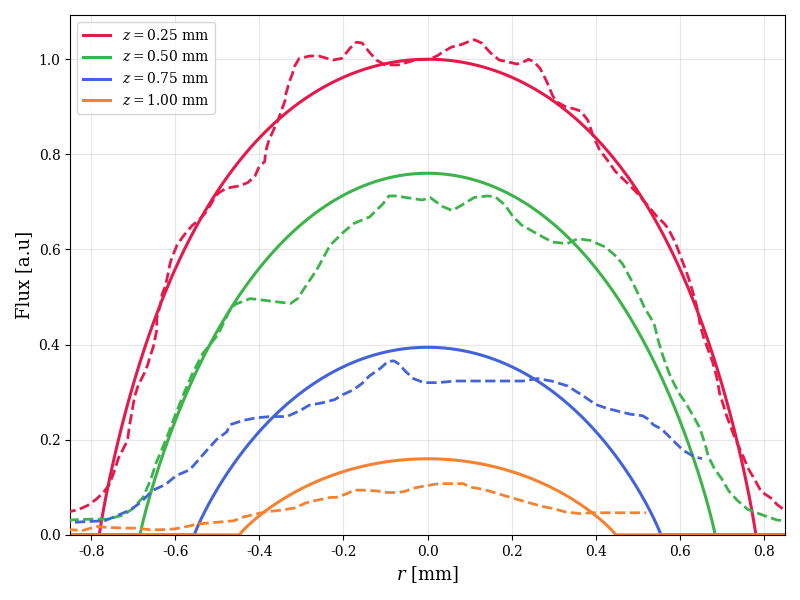
\includegraphics[width=\textwidth]{2D_model/flux_curvature_post_breakout_0.5ns.png}
        \end{column}
    \end{columns}
\end{frame}

% --- Section 4 ---
\section{Conclusion}
\begin{frame}{Conclusion}
    \begin{itemize}
        \item Summary of key findings
        \item Future work
    \end{itemize}
    \vspace{1cm}
    \begin{center}
        \Large \textbf{Thank You!} \\
        \vspace{0.5cm}
        \normalsize Questions?
    \end{center}
\end{frame}

\end{document}